%% expect: native native fallback native native fallback native
\documentclass{article}
\usepackage{tikz-cd}
\makeatletter
\newcommand\counts{\typeout{[[\the\pgf@picture@serial@count,\the\tikz@fig@count,\pgfpictureid,\meaning\tikzcdmatrixname,\the\pgfmatrixcurrentrow,\the\pgfmatrixcurrentcolumn]]}}
\makeatother
\begin{document}
\counts
\tikz \draw (0,0) -- (1,1);
\counts
\begin{tikzcd} A \arrow[r] & B \end{tikzcd}
\counts
\begin{tikzpicture} \node (x) {x}; \draw (x) -- (1,1); \end{tikzpicture}
\counts
\begin{tikzcd} A \arrow[r] & B \end{tikzcd}
\counts
\begin{tikzcd} A \arrow[r,execute at end to={}] & \tikz\draw (0,0) -- (1,0); \end{tikzcd}
\counts
\begin{tikzcd} A \arrow[r] & B \end{tikzcd}
\counts
\begin{tikzpicture}[remember picture,overlay] \draw (0,0) -- (1,1); \end{tikzpicture}
\counts
\begin{tikzcd} A \arrow[r] & B \end{tikzcd}
\counts
\begin{tikzcd}[remember picture] A \arrow[r] & B \end{tikzcd}
\counts
\begin{tikzcd} A \arrow[r] & B \end{tikzcd}
\counts
\begin{tikzpicture}[matrix of nodes] \matrix (m) {x \\}; \end{tikzpicture}
\counts
\end{document}
